% Background

Droidguardian was inspired by a powerful tool called \textit{Little Snitch}, that aims to raise awareness regarding internet connection attempts from the system's applications. Little Snitch provides a graphical interface so that users can filter outgoing internet connections\footnote{Later versions of Little Snitch allow to manage incoming internet connections as well, but this feature is out of this project scope.} through rules and accept or reject connections in real time. In order to develop Droidguardian, a deep study and understanding of Little Snitch took place and the following section will cover the relevant details. It might be important to stress the fact that Little Snitch is designed exclusively for Mac OS X operating system and it is not open source. All information presented below stems from both the use of the tool and available documentation reading.

Since Android is an embedded Linux environment product, in the initial research phase to design Droidguardian we stumbled upon a very interesting tool, quite similar to Little Snitch, although much simpler, called \textit{TuxGuardian}. This tool aims to exhibit in real time all outgoing internet connection attempts, allowing users to accept or reject such connections. TuxGuardian was designed for Linux based operating systems and is open source, which led to a thorough analysis introduced later in this chapter.

\section{Little Snitch}
\label{sec:little_snitch}

Little Snitch\footnote{http://www.obdev.at/products/littlesnitch/index.html} is by definition a firewall built for Mac OS X. However, it is not a regular firewall that operates at network packet level, checking protocol headers, but a firewall that acts at higher level, closer to the application layer. Little Snitch is set to intercept network connections attempts originated from all the system's applications and processes. Once a network connection attempt occurs in the system's kernel, it is intercepted by Little Snitch which will either accept it or reject it. This decision is based on a set of rules created by the user and by Little Snitch. The following section introduces Little Snitch rules.

\subsection{Little Snitch rules}

A rule is composed of four elements:

\begin{itemize}
\item Condition
\item Action
\item Lifetime
\item Annotations
\end{itemize}

When an application, or Unix process, tries to establish an internet connection, it passes to the system some required data, as an address and a port. These data is collected by Little Snitch that compares it to the existing rule. The \textit{condition} field of each rule has the following properties:

\begin{itemize}
 \item Process
 \item Process owner
 \item Server
 \item Port
 \item Protocol
 \item Direction
 \item Enabled
\end{itemize}

An internet connection might be seen as a triplet that includes a server, a port and a protocol. It has associated the process that triggered the connection and the owner of the process. The server is the remote internet address and Little Snitch handles them using numeric sets, \gls{dns} hostnames and \gls{dns} domains. The port points to services. Protocols (\gls{tcp}, \gls{udp} or \gls{icmp}) states the behavior of the internet connection. Processes are applications, as Safari, Mail, etc, and UNIX processes, as \textit{storeagent}, \textit{ntpd}, etc. These processes are owned by an entity, as System, root, etc. There are two other properties that belongs to conditions: connection direction and enabled. The first one indicates if the connection is incoming or outgoing and the last one may be seen as a flag that states if the rule is on or off.

Connection attempts are compared to these properties and, if a match occurs, the matched rule takes its action. A connection that matches an off enabled rule is not handled. The action is one of the following:

\begin{itemize}
 \item Allow
 \item Deny
 \item Ask
\end{itemize}

It's easy to understand that the rule may either allow or deny the connection. In the first case, the connection is established as if it was not intercepted by Little Snitch. In the second, the process attempting the connection receives an error, like a network failure, and the connection does not take place. The ask action is triggered when Little Snitch does not have the connection data stored, in a sequence of either being the first time the connection occurs or the user didn't want to save it earlier. Therefore, Little Snitch launches a dialog message, called \textit{Connection Alert}, reporting the connection attempt, revealing the connection properties and providing choice buttons so that the user may decide what to do. \autoref{fig:ls_dialog} shows a Little Snitch Connection Alert window. The figure reveals the Connection Summary, a short text indicating the server (\textit{ax.init.itunes.apple.com}), the port (\textit{80}) and the protocol (\textit{http}); the Action, composed by the choice buttons \textit{Allow} and \textit{Deny}; the Rule Lifetime, where the user assigns a time tag to the rule; Rule Options to determine if this application (\textit{iTunes}) is allowed to established every connection or if there are some restrictions regarding the server, port and protocol. At last, the Research Assist Button exhibits some detailed information about the connection's properties that may help users to decide what to do.

\begin{figure}[h]
 \begin{center}
 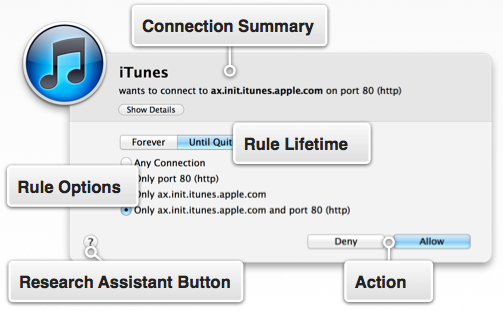
\includegraphics[scale=0.5]{figures/LS_Dialog.png}
 \end{center}
 \caption{Little Snitch Connection Alert window}
 \label{fig:ls_dialog}
\end{figure}

Rule Lifetime plays an important role. It allow users to define the frequency they want that connection to occur. He can choose one of the following tags:

\begin{itemize}
\item \textit{Forever} - The rule never expires;
\item \textit{Until Quit} - The rule expires when the last instance of the process that matches the rule terminates;
\item \textit{Until Logout} - The rule expires when the user who created the rule logs out;
\item \textit{Until Restart} - The rule expires when the computer is restarted;
\item \textit{Minutes} - The rule expires a certain amount of time after it was created;
\item \textit{Once} - The connection takes places and the rule is not saved.
\end{itemize}

The descriptions above explain how Little Snitch perform. For instance, a \textit{forever} rule will only display a Connection Alert once. All matching connections after the rule is setted up will be executed according to the action's rule. On the other side, if the user chooses the \textit{once} tag, is either allowing or denying the connection only this time and desires to be notified if it happen again. In this case, the Connection Alert will be prompt as if it was the first time this connection appears in the system.

As mentioned earlier, Little Snitch is a powerful tool. It has a mechanism to distinguish important processes that need to establish internet connections in order to keep the system executing without problems. These processes are automatically granted permission to connect to external servers. However, the user may check the related rules and change them. For this reason, Little Snitch provides the \textit{Annotation} field, in which rules are characterized as \textit{Protected} or \textit{Unapproved} to inform the user about their special status. Besides this feature, Little Snitch provides different profiles to each network the system is connected, and other useful features that make this tool quite robust and valuable.

\subsection{Little Snitch architecture}

A simple version of Little Snitch architecture is presented in \autoref{fig:ls_architecture}. At the bottom we find a Kernel Extension responsible for the interception of connection attempts. The ability to refuse an internet connection cannot be performed at user level. Therefore, Little Snitch developers was forced to operate at kernel level, building a Kernel Extension \cite{Documentation:LittleSnitch}. The collected data from the bottom layer is sent to the layer above, the Network Filter. The matching process is done in this layer. At the top is placed the user interface that permit users to check information, define rules, etc.

\begin{figure}[htbp]
 \centering
 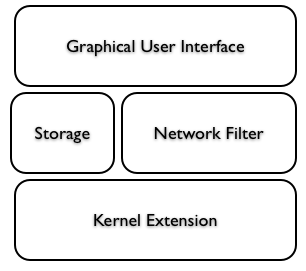
\includegraphics[scale=0.5]{figures/ls_arch.png}
 \caption{Little Snitch architecture}
 \label{fig:ls_architecture}
\end{figure}


% TuxGuardian

\section{TuxGuardian}
\label{sec:tuxguardian}

TuxGuardian\footnote{ http://tuxguardian.sourceforge.net} is an open source tool designed for Linux based operating systems, that intercepts outgoing internet requests and triggers notification alerts to the user. Its basic behavior is quite similar to Little Snitch. Although this tool stopped being updated since 2006, it was very important in the scope of this project and played a major role in Droidguardian's development process. In fact, that's where the name \textit{Droidguardian} came from. The following sections presents TuxGuardian in detail.

\subsection{TuxGuardian architecture}

TuxGuardian is a host firewall that emerged to overcome the complexity of Linux security model to lay users, providing an interface to implement access control policies to the network outgoing traffic. It consists of a three layered architecture showed in \autoref{fig:tg_architecture}. Each layer has a specific function and establishes a communication to the next layer. 

\begin{figure}[htbp]
 \centering
 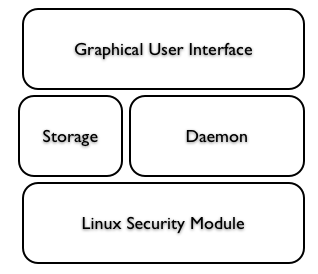
\includegraphics[scale=0.5]{figures/tg_arch.png}
 \caption{TuxGuardian architecture}
 \label{fig:tg_architecture}
\end{figure}

The \textit{Security Module} is the bottom layer and takes advantage of the \gls{lsm} framework  to implement hook functions that grab internet socket requests. Namely, TuxGuardian uses the callback functions \texttt{socket\_create} and \texttt{socket\_listen} to intercept both socket client and socket server internet connection requests\footnote{For the sake of simplicity, we will not cover security modules framework in this chapter, but it will be detailed later in this document.}. Local socket requests are not handled. Through this mechanism, TuxGuardian is able to block outgoing connections. In the same way as Little Snitch, this operation must be executed in kernel space. When the security module detects a connection attempt, sends a message to the layer above and waits a response in order to either deny or allow the connection.

The \textit{Daemon} is by definition a program that executes in background waiting for some event to take place. In this case, it waits for the security module messages, that consists of the \gls{pid} of the process that created the connection request. This communication process is established through local sockets. When the daemon gets the security module's message, checks the storage file to find a connection match. This procedure is also very similar to Little Snitch. If a match is found, TuxGuardian executes the corresponding action. Otherwise, it launches a notification window to get the user's response. Note that TuxGuardian is able to perform without the \gls{gui} component, denying all connections that are not placed in the storage file. In order to enforce a security measure, TuxGuardian keeps the MD5 hash of each process path. Through \gls{pid}s, the daemon gets the process path name in the \texttt{/proc} directory and calculates its MD5 hash so that modified programs cannot access internet.

The \gls{gui} or \textit{Frontend} displays the notification windows. The user receives the process name (the complete process path, for instance \texttt{/bin/ping}) that created the connection attempt and decides to either accept it or reject it. Along with the process path, the corresponding MD5 hash is also displayed. \autoref{fig:tg_dialog} presents the TuxGuardian notification window.

\begin{figure}[h]
 \begin{center}
 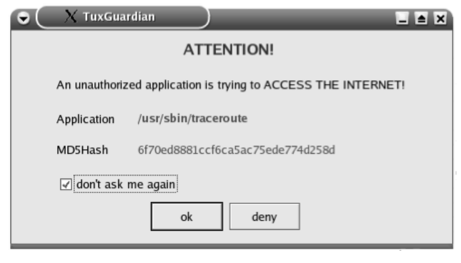
\includegraphics[scale=0.5]{figures/tg_dialog.png}
 \end{center}
 \caption{TuxGuardian notification window}
 \label{fig:tg_dialog}
\end{figure}

\subsection{TuxGuardian Protocol}

The communication between layers is established through the \gls{tgp} \cite{Report:TuxGuardian}. This comprises a structure with the following fields:

\begin{itemize}
\item Sender
\item Sequence number
\item Query type
\item Query data
\end{itemize}

\textit{Sender} specifies the layer which sent the message: 

\begin{itemize}
\item \texttt{TG\_MODULE},
\item \texttt{TG\_DAEMON},
\item  \texttt{TG\_FRONTEND}
\end{itemize}

corresponding to the security module, the daemon and the frontend, respectively. \textit{Sequence number} acts as the message identifier. \textit{Query type} characterizes the message, or query, as follows:

\begin{itemize}
\item \texttt{TG\_ASK\_PERMIT\_APP} refers to the query sent by the security module to the daemon asking permission to either allow or deny the connection request;
\item \texttt{TG\_RESPOND\_PERMIT\_APP} refers to the response the security module gets from the daemon to the question above. \textit{Query data} field stores the permission value;
\item \texttt{TG\_PERMIT\_SERVER} refers to the first query, but indicating that the connection request involves a server;
\item \texttt{TG\_RESPOND\_PERMIT\_SERVER} refers to the response obtained from the previous question.
\end{itemize}

Depending on the nature of the query, \textit{Query data} may store a \gls{pid} or the permission values: either \textit{yes} or \textit{no}. 